\chapter{Découvrons Xcode}
Dans cette parte nous allons installer et découvrir l'IDE d’Apple, puis découvrir notre
première ligne de code.
\section{Installation de Xcode}
L'installation de cet outil est plutôt facile, puisqu’il est disponible depuis le Mac app Store,
gratuitement. On peux aussi le télécharger depuis le site des développeurs Apple. Il faut
cependant s'inscrire en tant que développeur avec son Apple ID, gratuitement, pour
accéder aux divers ressource, dont la documentation, je vous recommande donc de le
faire.
(Attention , les programmes payants ne sont pas nécessaires, il servent juste à pouvoir
soumettre des applications sur les App Store, et pouvoir signer son code, pour la
distribution via internet)
Une fois les quelques Giga-octets de l'application téléchargés (grosse pause café), vous
verrez l'application apparaitre dans votre dossier application.
\begin{figure}[h]
\centering
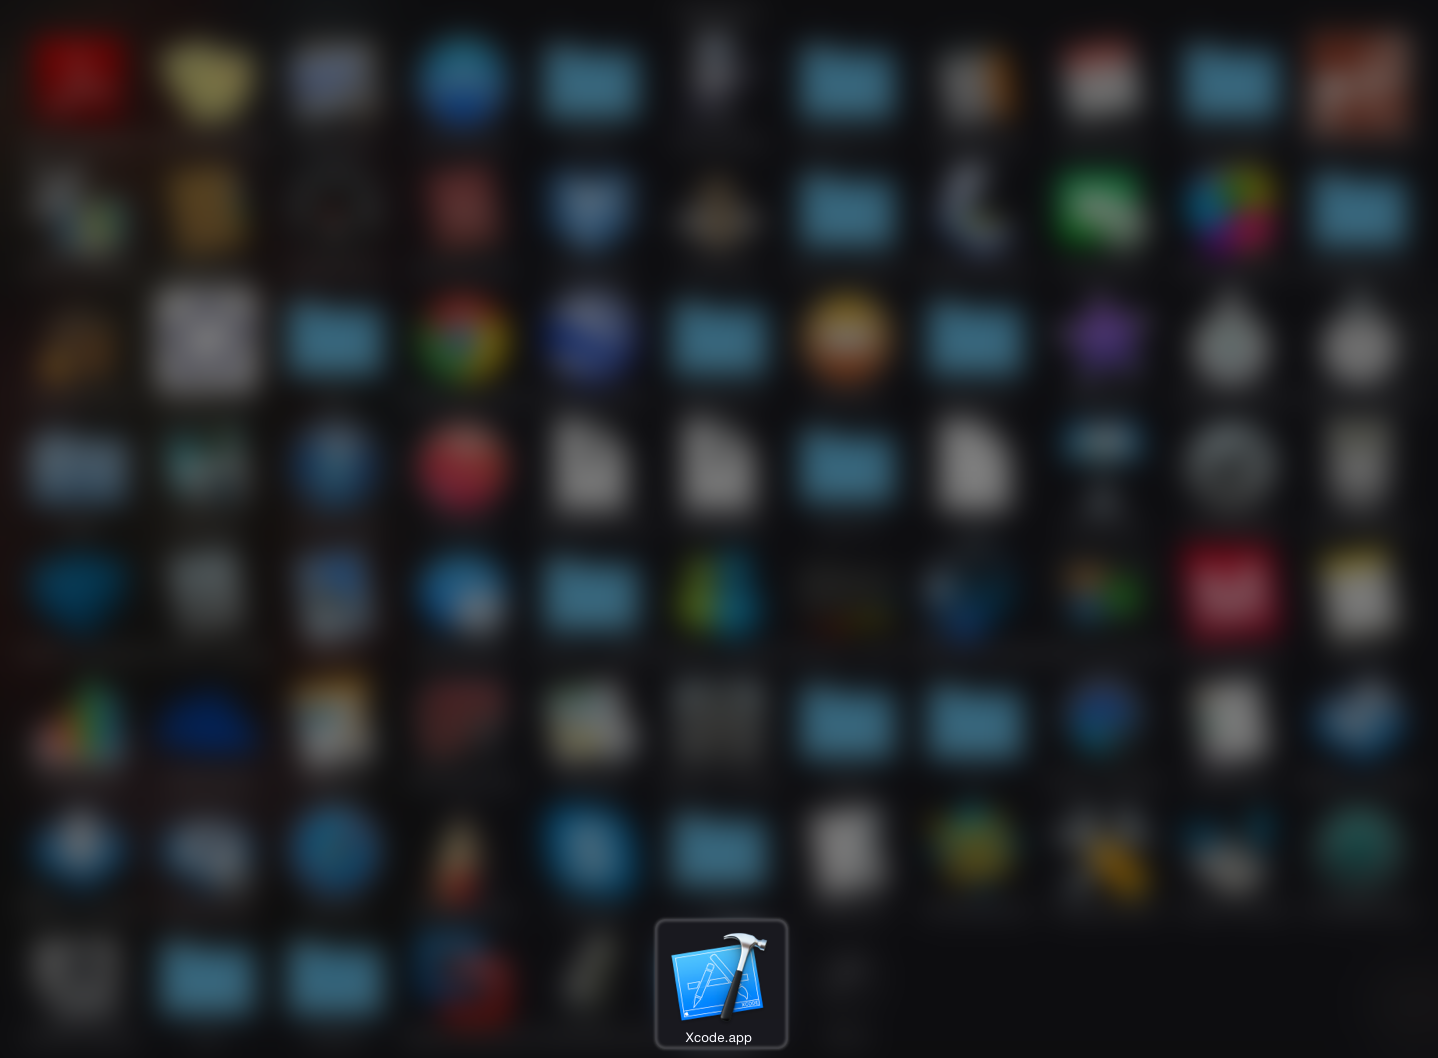
\includegraphics[scale=0.30]{\TSwiftRoot/P1/CH2/img/Launchpad}
\caption{L'icône de Xcode dans la pile Applications}
\end{figure}

\section{Premier contact avec Swift, un Playground}
Ouvrez Xcode. Vous devez voir apparaitre cette fenêtre, à la colonne de droite près.
\begin{figure}[h]
\centering
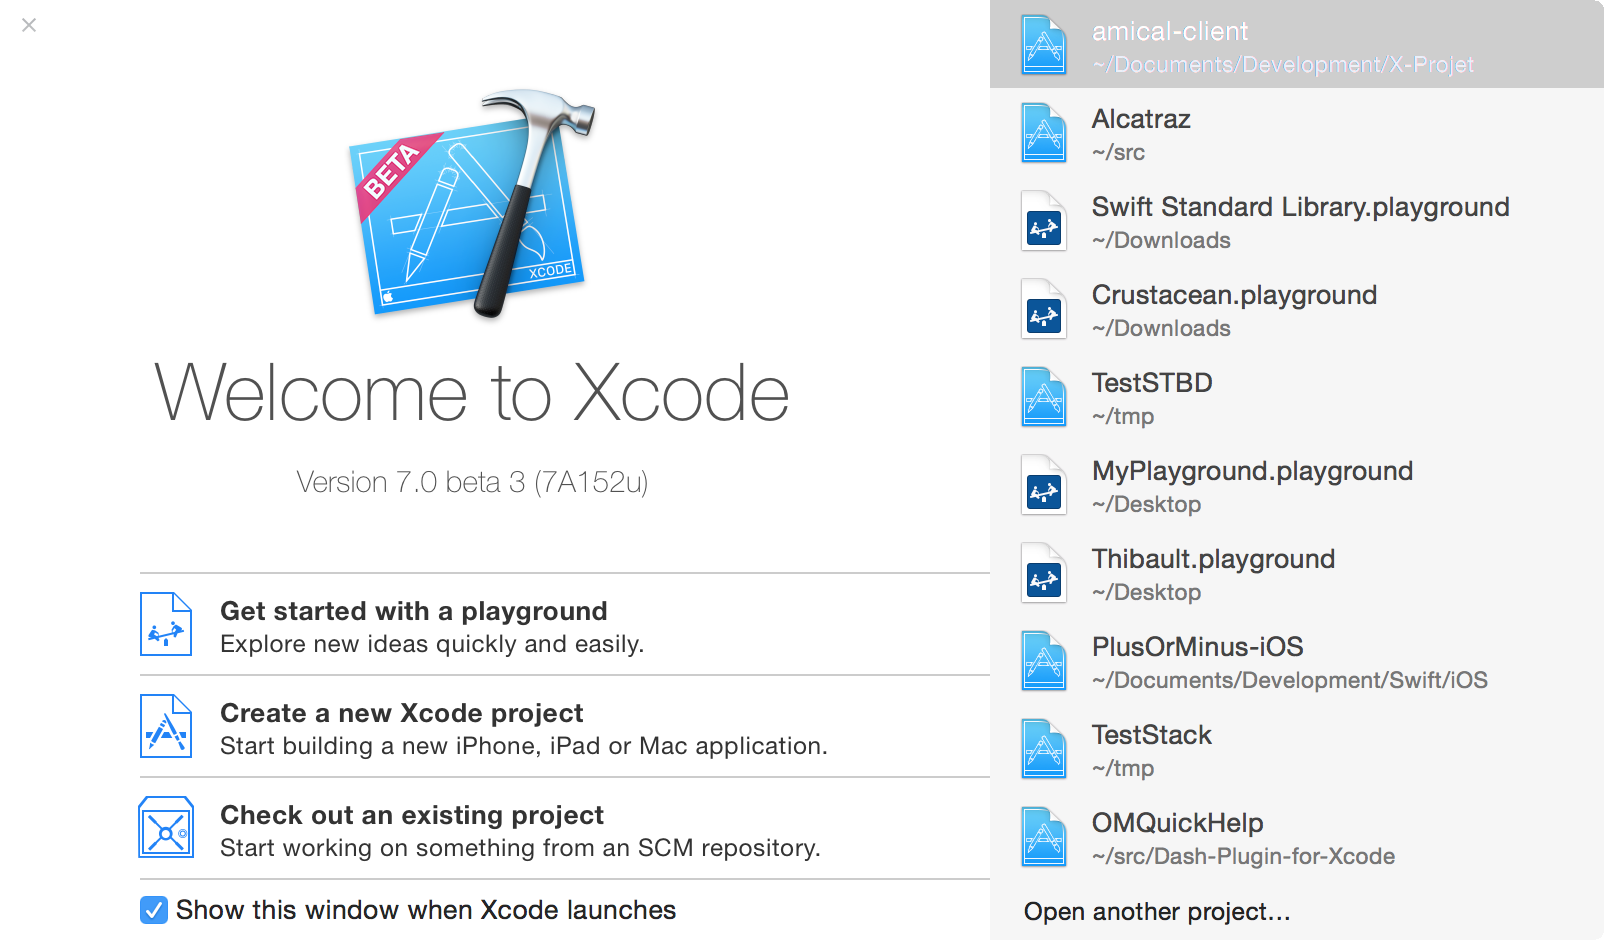
\includegraphics[scale=0.5]{\TSwiftRoot/P1/CH2/img/XCodeWindow}
\caption{Fenêtre d'accueil de Xcode}
\end{figure}

Cliquez sur << Get started with a playground >>, pour créer un nouveau playground.
Choisissez comme plateforme OS X, et donnez lui un nom sensé.
Une fois le projet enregistré, vous voyez apparaitre une fenêtre en deux parties.
A gauche un éditeur de texte qui contient du code Swift, à droite une colonne dans
laquelle sont affichés les résultats de chaque instructions.
En Swift une instruction se termine par un retour à la ligne, ou un point virgule (Si on tient
absolument à mettre plusieurs instructions sur une ligne).
Vous avez normalement le code suivant, affichant \verb"Hello, playground" en face de la troisième ligne :
\begin{listing}[h]
\caption{Code par défaut d'un Playground Swift}
\begin{minted}[linenos=true]{swift}
// Playground - noun: a place where people can play

import Cocoa

var str = "Hello, playground"
\end{minted}
\end{listing}

Remplacez le par le code suivant :
\begin{listing}[h]
\caption{Programme affichant "Hello, playground"}
\begin{minted}[linenos=true]{swift}
// Playground - noun: a place where people can play

println("Hello, playground")
\end{minted}
\end{listing}

Ce code semble avoir le même effet que le précédent, mais cela n'est vrai que dans un playground, qui est un environnement très particulier.

Il s’agit du premier programme que l’on montre par convention dans un nouveau langage :
« Hello, World ! », qui affiche à l’écran le texte en question.

La première ligne de code est un commentaire (ignoré royalement par le compilateur)
notion que nous étudieront dans la prochaine partie, la deuxième la ligne qui affiche le
texte << Hello, Playground ! >> (sans les guillemets à l’écran).
On reviendra plus en détail sur cette ligne plus tard, mais je tenait à vous présenter ce
programme, qui est plutôt court dans ce langage (1 ligne en Swift, contre 4 lignes en C).

Vous pouvez remplacer le texte entre guillemet par le texte que vous voulez.

println est la fonction qui est chargé d’afficher à l’écran une ligne de texte.

Cette ligne de code correspond à une instruction.
Un playground est un outil très puissant de Xcode puisqu’il permet de voir immédiatement
les conséquences d’une modification du code.
\section{Les Commentaires}
Un commentaire permet à l’auteur du code d’expliquer ce qu’il fait, ou plus généralement
d’introduire dans le code source du texte ignoré par le compilateur.

Vous allez me dire, que vous ne voyez pas à quoi cela sert. En fait, lire le code d’un autre
programmeur n’est pas toujours évident, (à quoi ça sert ça !? Et qu’est ce que tu veux faire
là ?). Pour aider les autres, et soi même, lorsqu’on se replonge dans son code des mois après, il est donc
indispensable d’expliquer son code.

Comme un court exemple vaut mieux qu’un long discours je vous laisse consulter le code.

\emph{Attention à ceux qui connaissent les commentaires du C, en Swift, les commentaires
s'imbriquent les un dans les autres.}

\begin{listing}[h]
\caption{Que de commentaires !}
\begin{minted}[linenos=true]{swift}
// Ceci est un commentaire s'arrêtant en fin de ligne.
/* Ceci est un commentaire qui s'arrête au symbole */
/*
Il peut s'étendre sur plusieurs lignes
// Je suis un commentaire imbriqué
/*Moi aussi*/
println("Hello, playground")
Mais rien ne se passe !
Fin du commentaire sur plusieurs lignes:*/
// On peut placer un commentaire après une instruction
println("Hello, playground") // Comme ici.
// Ou même au milieu
println(/*Texte ici*/"Bonjour, bac à sable") // Parce qu'en Français c'est mieux.
\end{minted}
\end{listing}
Remarquez que Xcode colore les commentaires d'une couleur particulière (chez moi, le vert).
\section{Un quasi-interpréteur : La REPL Swift}
Le playground, est un outil très puissant puisqu’il compile et exécute immédiatement
chacune de vos instructions.

En arrière plan, Xcode compile automatiquement votre programme, et utilise le debugger
pour obtenir l’état du programme après chaque instruction.

Il existe une autre façon de jouer avec Swift, un peu moins jolie mais encore plus rapide
qu’un playground qui reste un fichier : La << Read Eval Print Loop >>, boucle de lecture évaluation écriture, basé elle aussi sur le
débugger. Si vous avez déjà utilisé la ligne de commande ou utilisé un langage interprété
comme Python, je vous la présente ici, sinon vous pouvez sauter cette partie, ou vous
référer au tutoriel OSX ici \url{http://openclassrooms.com/courses/domptez-votre-mac-avec-os-x-yosemite/le-terminal-dans-os-x-1}.

Ouvrez un Terminal Unix, et tapez \verb"swift".
Tapez ensuite une ligne de code et appuyez sur entrée.
swift affiche alors le résultat.
Pour quitter tapez \verb":quit".
En arrière plan Swift compile la ligne de code puis l'exécute et affiche le résultat.
Attention, contrairement à un interpréteur qui lit la ligne dans son langage et exécute
les instructions en question, il y a bien ici création du code binaire correspondant.
Cet outil peut être très puissant, mais je ne le détaillerai pas ici, libre à vous de l’explorer.
\begin{listing}[h]
\caption{Exemple de sortie après un usage de la REPL Swift}
\begin{verbatim}
$ swift
Welcome to Swift!  Type :help for assistance.
  1> println("Hello, REPL")
Hello, REPL
  2> :quit
$
\end{verbatim}
% Check if this is correct.
\end{listing}